\section{Not\-Redundant$<$ Data, Attribute\-Type, Measure, f, Cand\_\-Data\-Struct $>$ Class Template Reference}
\label{class_not_redundant}\index{NotRedundant@{NotRedundant}}
Functor representing the predicate being not redundant.  


{\tt \#include $<$Not\-Redundant.hxx$>$}

Inheritance diagram for Not\-Redundant$<$ Data, Attribute\-Type, Measure, f, Cand\_\-Data\-Struct $>$::\begin{figure}[H]
\begin{center}
\leavevmode
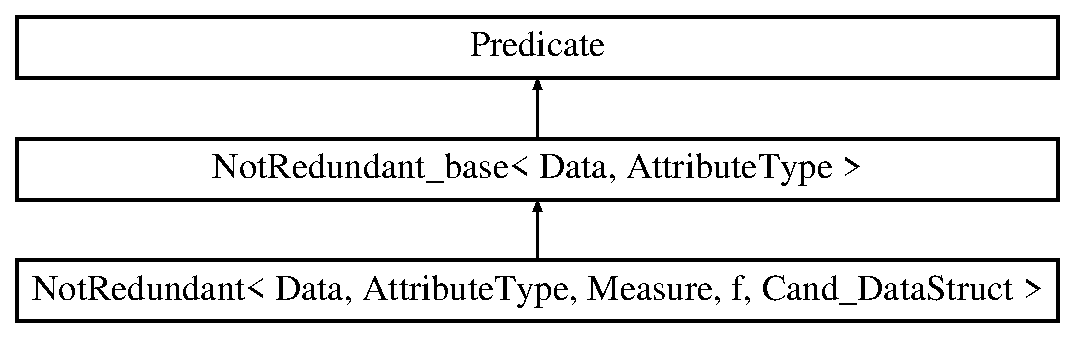
\includegraphics[height=3cm]{class_not_redundant}
\end{center}
\end{figure}
\subsection*{Public Member Functions}
\begin{CompactItemize}
\item 
template$<$class Input\-DBFormat$>$ {\bf Not\-Redundant} (Data \&intable, Input\-DBFormat \&input)\label{class_not_redundant_9c9b80eb14297e25c3fe673143518d48}

\begin{CompactList}\small\item\em Constructor. \item\end{CompactList}\item 
{\bf $\sim$Not\-Redundant} ()\label{class_not_redundant_7c0d90edb6ba88c1f88917ce435c119f}

\begin{CompactList}\small\item\em Destructor. \item\end{CompactList}\item 
bool {\bf operator()} ({\bf Iterator\-Cand} \&itemset\-It, Measure \&meas\-Cand)
\begin{CompactList}\small\item\em Operator that test if a set of attributes is not redundant. \item\end{CompactList}\item 
void {\bf pre\-Processing} (Cand\_\-Data\-Struct \&cand\-Set, f inword\-To\-Set)\label{class_not_redundant_f5217ca7c07b87ac2a051ce4b004734d}

\begin{CompactList}\small\item\em Function used to count the projection of the elements in the data. \item\end{CompactList}\end{CompactItemize}


\subsection{Detailed Description}
\subsubsection*{template$<$class Data, class Attribute\-Type, class Measure, class f = Id, class Cand\_\-Data\-Struct = PTree$<$Attribute\-Type,Measure$>$$>$ class Not\-Redundant$<$ Data, Attribute\-Type, Measure, f, Cand\_\-Data\-Struct $>$}

Functor representing the predicate being not redundant. 

This functor test if an itemset is not redundant. In this class, the test method is optimized for candidates in a {\bf PTree}{\rm (p.\,\pageref{class_p_tree})} data structure. If the iterator passed in parameter of the functor is not an iterator on a {\bf PTree}{\rm (p.\,\pageref{class_p_tree})}, the functor use a non optimized method.

This functor process and count the projection BEFORE pruning. This version of the predicate store the cardinality of the projection with the candidates. For each candidate tested, this predicate does not count the projection of all the subsets, and instead use the values stored. This suppose that all the subsets have been generated, tested ad stored. The template parameter Data is the type of the tablular data. 



\subsection{Member Function Documentation}
\index{NotRedundant@{Not\-Redundant}!operator()@{operator()}}
\index{operator()@{operator()}!NotRedundant@{Not\-Redundant}}
\subsubsection{\setlength{\rightskip}{0pt plus 5cm}template$<$class Data, class Attribute\-Type, class Measure, class f, class Cand\_\-Data\-Struct$>$ bool {\bf Not\-Redundant}$<$ Data, Attribute\-Type, Measure, f, Cand\_\-Data\-Struct $>$::operator() ({\bf Iterator\-Cand} \& {\em itemset\-It}, Measure \& {\em meas\-Cand})}\label{class_not_redundant_11c7c4da4c46bbb5cd2546fc07801b32}


Operator that test if a set of attributes is not redundant. 

This operator is optimized for the case where the set of candidate is a trie data structure (PTree), and for each set tested all his subsets have been already tested (their projection is counted). Typicaly this method is used when we have an algorithm we a bottom up exploration of the search space such as {\bf Apriori}{\rm (p.\,\pageref{class_apriori})}.

\begin{Desc}
\item[Parameters:]
\begin{description}
\item[{\em itemset\-It}]iterator (or pointer) on the itemset to test wrt the predicate \item[{\em mes\-Cand}]value of the support of the itemset \end{description}
\end{Desc}


The documentation for this class was generated from the following file:\begin{CompactItemize}
\item 
D:/Implementations/Librairie/problems/not\-Redundant/Not\-Redundant.hxx\end{CompactItemize}
